\documentclass[presentation]{beamer}

\usepackage{tikz}
\usetikzlibrary{positioning,calc}
\usetikzlibrary{shapes.geometric}
\usetikzlibrary{backgrounds}% only to show the bounding box
\usetikzlibrary{shapes,arrows}
\usepackage{pgfplots}
\usepackage{pgfplotstable}
\usetikzlibrary{pgfplots.groupplots}
\pgfplotsset{compat=1.12}
\usepackage{appendixnumberbeamer}
\usepackage{amsmath}
\usepackage[utf8]{inputenc}
\date{28th March 2017}
\usetheme{firedrake}

\renewcommand{\vec}[1]{\ensuremath{\boldsymbol{#1}}}
\newcommand{\ddt}[1]{\frac{\partial #1}{\partial t}}
\newcommand{\zhat}{\hat{\vec{z}}}
\newcommand{\W}{\ensuremath{\mathbb{W}}}

\newcommand{\inner}[1]{\left\langle #1 \right \rangle}

\newcommand{\KSP}[2]{\ensuremath{\mathcal{K}\left(#1, \mathbb{#2}\right)}}
\newcommand{\ksp}[1]{\KSP{#1}{#1}}

\newcommand{\highlight}[1]{\colorbox{red!20}{\color{black} #1}}

\author{Lawrence Mitchell\inst{1,*} \and Rob Kirby\inst{2}}
\institute{
\inst{1}Departments of Computing and Mathematics, Imperial College
London

\inst{*}\texttt{lawrence.mitchell@imperial.ac.uk}
\and
\inst{2}Department of Mathematics, Baylor University
}

\graphicspath{{./\jobname.figures/}}

\usepackage[url=false,
            doi=true,
            isbn=false,
            style=authoryear,
            firstinits=true,
            uniquename=init,
            backend=biber]{biblatex}

\setbeamertemplate{bibliography item}{}
\renewcommand{\bibfont}{\fontsize{7}{7}\selectfont}
\addbibresource{references.bib}
\newcommand{\arxivlink}[2]{%
  \href{http://www.arxiv.org/abs/#1}%
  {{\small\texttt{arXiv:\,#1\,[#2]}}}%
}

\setlength{\bibitemsep}{1ex}
\setlength{\fboxsep}{1pt}

\renewbibmacro{in:}{}
\DeclareFieldFormat[article]{volume}{\textbf{#1}}
\DeclareFieldFormat{doi}{%
  doi\addcolon%
  {\ifhyperref{\href{http://dx.doi.org/#1}{\nolinkurl{#1}}}
    {\nolinkurl{#1}}}}
\AtEveryBibitem{%
\clearfield{pages}%
\clearfield{issue}%
\clearfield{number}%
}

\usepackage{minted}

\title{Across the great divide}
\subtitle{composable block preconditioning from UFL}
\begin{document}

\maketitle

\begin{frame}[fragile]
  \frametitle{UFL makes it easy to write complex PDEs}
  \begin{columns}
    \begin{onlyenv}<1>
      \begin{column}{0.47\framewidth}
        \small
      \begin{block}{Rayleigh-B\'enard convection}
        \begin{equation*}
          \begin{split}
            -\Delta u + u\cdot\nabla u + \nabla p +
            \frac{\text{Ra}}{\text{Pr}} \hat{g}T &= 0 \\
            \nabla \cdot u &= 0 \\
            - \frac{1}{\text{Pr}} \Delta T + u\cdot \nabla T &= 0
          \end{split}
        \end{equation*}
      \end{block}
    \end{column}
    \begin{column}{0.52\framewidth}
\begin{minted}[fontsize=\tiny]{python}
from firedrake import *
mesh = Mesh(...)
V = VectorFunctionSpace(mesh, "CG", 2)
W = FunctionSpace(mesh, "CG", 1)
Q = FunctionSpace(mesh, "CG", 1)
Z = V * W * Q
upT = Function(Z)
u, p, T = split(upT)
v, q, S = TestFunctions(Z)
bcs = [...] # no-flow + temp gradient
nullspace = MixedVectorSpaceBasis(
   Z, [Z.sub(0), VectorSpaceBasis(constant=True), 
       Z.sub(2)])
F = (inner(grad(u), grad(v))
     + inner(dot(grad(u), u), v)
     - inner(p, div(v))
     + (Ra/Pr)*inner(T*g, v)
     + inner(div(u), q)
     + inner(dot(grad(T), u), S)
     + (1/Pr) * inner(grad(T), grad(S)))*dx

solve(F == 0, upT, bcs=bcs, nullspace=nullspace)
\end{minted}
    \end{column}
  \end{onlyenv}
  \end{columns}
\end{frame}

\begin{frame}[fragile]
  \begin{columns}
    \begin{column}{0.5\textwidth}
      \begin{block}{Ohta-Kawasaki}
        \small
        \begin{align*}
          u_t - \Delta w + \sigma(u - m) &= 0\\
          w + \epsilon^2 \Delta u - u(u^2 - 1) &= 0
        \end{align*}
        Implicit timestepping + Newton
        \begin{equation*}
          \begin{bmatrix}
            (1 + \Delta t \theta \sigma)M  & \Delta t\theta K \\
            -\epsilon^2 K - M_E & M
          \end{bmatrix}
          \begin{bmatrix}
            \delta u \\
            \delta w
          \end{bmatrix} =
          \begin{bmatrix}
            f_1 \\
            f_2
          \end{bmatrix}
        \end{equation*}
      \end{block}
    \end{column}
    \begin{column}{0.5\textwidth}
\begin{minted}[fontsize=\tiny,escapeinside=||]{python}
from firedrake import *
|$\epsilon$| = Constant(0.02)
|$\sigma$| = Constant(100)
dt = Constant(eps**2)
|$\theta$| = Constant(0.5)
mesh = Mesh(...)
V = FunctionSpace(mesh, "CG", 1)
Z = V*V
v, q = TestFunctions(Z)
z = Function(Z)
z0 = Function(Z)
u, w = split(z)
u0, w0 = split(z0)
u|$_\theta$| = (1 - |$\theta$|)*u0 + |$\theta$|*u
w|$_\theta$| = (1 - |$\theta$|)*w0 + |$\theta$|*w
dfdu = u**3 - u
L = ((u - u0)*v
     + dt*dot(grad(w|$_\theta$|), grad(v))
     + dt*|$\sigma$|*(u|$_\theta$| - m)*v
     + w*q - dfdu*q
     - |$\epsilon$|**2*dot(grad(u), grad(q)))*dx
while t < Tend:
   z0.assign(z)
   solve(L == 0, z)
\end{minted}
    \end{column}
  \end{columns}
\end{frame}

\begin{frame}[fragile]
  \begin{columns}
    \begin{column}{0.5\textwidth}
      \begin{block}{Cahn-Hilliard}
        \small
        \begin{align*}
          \phi_t - \nabla \cdot M \nabla \mu &= 0\\
          \mu - \frac{\text{d} f}{\text{d} \phi} + \lambda \Delta \phi &= 0\\
        \end{align*}
        Implicit timestepping
        \begin{equation*}
          \begin{bmatrix}
            \frac{\phi_{n+1} - \phi_n}{\Delta t} - \nabla \cdot M \nabla \mu_{n+\theta}\\
            \mu_{n+1} - \frac{\text{d} f_{n+1}}{\text{d} \phi_{n+1}} -
            \lambda \nabla^2\phi_{n+1}
          \end{bmatrix} = 0
        \end{equation*}
      \end{block}
    \end{column}
    \begin{column}{0.5\textwidth}
\begin{minted}[fontsize=\tiny,escapeinside=||]{python}
from firedrake import *
mesh = Mesh(...)
V = FunctionSpace(mesh, "CG", 1)
Z = V*V
|$\theta$| = 0.5
|$\lambda$| = Constant(0.005)
M = Constant(10)
q, v = TestFunctions(Z)
z = Function(Z)
z0 = Function(Z)
|$\phi_{n+1}$|, |$\mu_{n+1}$| = split(z)
|$\phi_n$|, |$\mu_n$| = split(z0)
|$\phi_{n+1}$| = variable(|$\phi_{n+1}$|)
f = 10*(|$\phi_{n+1}$|**2 - 1)**2
dfdphi = diff(f, |$\phi_{n+1}$|)
|$\mu_{n+\theta}$| = (1-|$\theta$|)*|$\mu_n$| + |$\theta$|*|$\mu_{n+1}$|
dt = 5e-6
F = ((|$\phi_{n+1}$| - |$\phi_n$|)*q 
     + dt*M*dot(grad(|$\mu_{n+\theta}$|), grad(q)) 
     + (|$\mu_{n+1}$| - dfdphi)*v
     -|$\lambda$|*dot(grad(|$\phi_{n+1}$|), grad(v)))*dx
while t < tEnd:
    z0.assign(z)
    solve(F == 0, z)
\end{minted}
    \end{column}
  \end{columns}
\end{frame}

\begin{frame}[t]
  \frametitle{What about the solvers?}
  \begin{itemize}
  \item LU is alright for small problems
  \item \dots but quickly becomes untenable in 3D.
  \item Instead we use iterative methods (e.g. Krylov methods)
  \item<2-> \dots but Krylov methods are \emph{not} solvers
  \item<3-> so we need \emph{preconditioners}.
  \end{itemize}
\end{frame}
\begin{frame}
  \frametitle{Block preconditioning}
  \begin{itemize}
  \item Coupled problems are (typically) not amenable to black
    box preconditioning.
  \item<2-> Solution: block preconditioning
  \end{itemize}
  \begin{columns}<2>[t]
    \begin{column}{0.5\textwidth}
      \begin{block}{Schur complement}
        \begin{equation*}
          T = \begin{bmatrix}
            A & 0 \\
            0 & C A^{-1} B^T
          \end{bmatrix}^{-1}
          \begin{bmatrix}
            A & B^T \\
            C & D = 0
          \end{bmatrix}
        \end{equation*}
        has minimal polynomial $T(T - I)(T^2 - T - I) = 0$.
        \nocite{Murphy:2000,Ipsen:2001,Benzi:2005}
      \end{block}
    \end{column}
    \hspace{1em}
    \begin{column}{0.5\textwidth}
      \begin{block}{Function space}
        If $\mathcal{A} : W \rightarrow W^*$, then
        \begin{equation*}
          \langle u, v \rangle_W^{-1} \mathcal{A}
        \end{equation*}
        has mesh independent condition number.
        \nocite{Malek:2014,Mardal:2011,Kirby:2010}
      \end{block}
    \end{column}
  \end{columns}
\end{frame}

\begin{frame}
  \frametitle{A problem}
  \begin{itemize}
  \item Such preconditioners often need auxiliary matrices not
    appearing the original operator.
  \item How do we provide these to the solver library in a composable
    manner?
  \end{itemize}
  \begin{block}<2->{Firedrake \& PETSc to the rescue}
  \begin{itemize}
  \item PETSc already provides a highly runtime-configurable library
    for \emph{algebraically} composing solvers \parencite{Brown:2012}.

  \item Firedrake makes it straightforward to build auxiliary
    operators.

  \item We combine these to allow simple development of complex
    preconditioners.
  \end{itemize}
  \end{block}
\end{frame}
\begin{frame}
  \frametitle{Two new pieces}
 
  \begin{onlyenv}<1>
    \begin{block}{A new matrix type}
      A PETSc shell matrix that implements matrix-free actions using
      Firedrake, and contains the UFL of the bilinear form.
      \begin{equation*}
        y \leftarrow A x
      \end{equation*}
    \end{block}
  
    \begin{block}{Custom preconditioners}
      These matrices do not have entries, so we create preconditioners
      that can inspect the UFL and do the appropriate thing.
      \begin{equation*}
        y \leftarrow \tilde{A}^{-1} x
      \end{equation*}
    \end{block}
  \end{onlyenv}
  \begin{onlyenv}<2>
    \begin{center}
      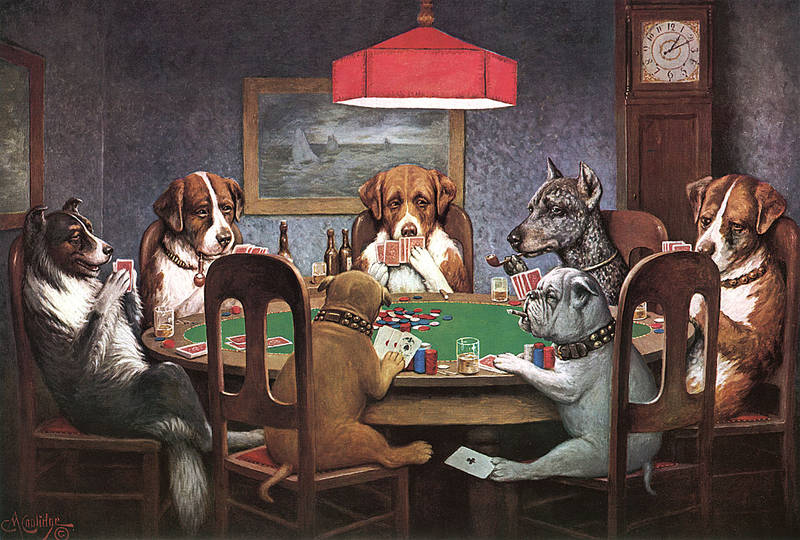
\includegraphics[width=0.8\textwidth]{underhand}
    \end{center}
  \end{onlyenv}
\end{frame}

\begin{frame}[allowframebreaks]
  \frametitle{An example}
  A preconditioner for the Ohta--Kawasaki
  equation \parencite{Farrell:2016}

  \begin{equation*}
    \begin{split}
      u_t - \Delta w + \sigma(u - m) &= 0\\
      w + \epsilon^2 \Delta u - u(u^2 - 1) &= 0
    \end{split}
  \end{equation*}
  Newton iteration at each timestep solves
  \begin{equation*}
    \begin{bmatrix}
      (1 + \Delta t \theta \sigma)M  & \Delta t\theta K \\
      -\epsilon^2 K - M_E & M
    \end{bmatrix}
    \begin{bmatrix}
      \delta u \\
      \delta w
    \end{bmatrix} =
    \begin{bmatrix}
      f_1 \\
      f_2
    \end{bmatrix}
  \end{equation*}

  \pagebreak
  
  Preconditioning
  \begin{equation*}
    P^{-1} = 
    \begin{bmatrix}
      (1 + \Delta t \theta \sigma)M  & 0 \\
      -\epsilon^2 K - M_E & S
    \end{bmatrix}^{-1} =
    \begin{bmatrix}
      A^{-1}  & 0 \\
      0 & S^{-1}
    \end{bmatrix}
    \begin{bmatrix}
      I & 0 \\
      -C A^{-1}  & I
    \end{bmatrix}.
  \end{equation*}
  Use
  \begin{equation*}
    S^{-1} \approx \hat{S}^{-1}M\hat{S}^{-1}
  \end{equation*}
  where
  \begin{equation*}
    \hat{S} = M + \epsilon\sqrt{(\Delta t \theta)/(1+\Delta t \theta\sigma)} K.
  \end{equation*}
\end{frame}

\begin{frame}
  \frametitle{A tree of solvers}
  \footnotesize
  \begin{equation*}
    J \triangleq \begin{bmatrix}
      (1 + \Delta t \theta \sigma)M  & \Delta t\theta K \\
      -\epsilon^2 K - M_E & M
    \end{bmatrix} \triangleq
    \begin{bmatrix}
      A & B \\
      C & M
    \end{bmatrix}
  \end{equation*}
  \begin{equation*}
    J^{-1} \approx \mathcal{K}\left(\begin{bmatrix}
        A  & B \\
        C & M
      \end{bmatrix},
      \begin{bmatrix}
        \mathcal{K}(A, A_p) & 0\\
        0 & \mathcal{K}(S, S_p)
      \end{bmatrix}
      \begin{bmatrix}
        I & 0\\
        -C\mathcal{K}(A, A_p) & I
      \end{bmatrix}\right)
  \end{equation*}
  \begin{align*}
    S &\triangleq M - C\mathcal{K}(A, A_p)B\\
    S_p &\triangleq \mathcal{K}(\hat{S}, \hat{S}_p)M\mathcal{K}(\hat{S}, \hat{S}_p)\\
    \hat{S} &\triangleq M + \epsilon\sqrt{(\Delta t \theta)/(1+\Delta t \theta\sigma)} K.
  \end{align*}
\end{frame}
\begin{frame}[fragile]
  \frametitle{Implementation}
\begin{minted}[fontsize=\tiny,mathescape,escapeinside=||]{python}
class OKPC(PCBase):

    def initialize(self, pc):
        # Approximate $S^{-1} \sim \hat{S}^{-1} M \hat{S}^{-1}$ where $\hat{S} = \inner{q, w} + \epsilon\sqrt{c}\inner{\nabla q, \nabla w}$
        _, P = pc.getOperators()
        ctx = P.getPythonContext()
        # User information about $\Delta t$, $\theta$, etc...
        dt, |$\theta$|, |$\epsilon$|, |$\sigma$| = ctx.appctx["parameters"]
        V = ctx.a.arguments()[0].function_space()
        c = (dt * |$\theta$| * |$\epsilon$|**2)/(1 + dt * |$\theta$| * |$\sigma$|)
        w = TrialFunction(V)
        q = TestFunction(V)
        op = assemble(inner(w, q)*dx + |$\epsilon$|*sqrt(c) * inner(grad(w), grad(q))*dx)
        self.ksp = KSP().create(comm=pc.comm)
        self.ksp.setOptionsPrefix(pc.getOptionsPrefix + "shat_")
        self.ksp.setOperators(op.petscmat, op.petscmat)
        [...] # boilerplate elided
        mass = assemble(w*q*dx)
        self.mass = mass.petscmat
        work = self.mass.createVecLeft()
        self.work = (work, work.duplicate())

    def apply(self, pc, x, y):
        tmp1, tmp2 = self.work
        self.ksp.solve(x, tmp1)
        self.mass.mult(tmp1, tmp2)
        self.ksp.solve(tmp2, y)
\end{minted}
\end{frame}

\begin{frame}[fragile]
  \frametitle{Usage}
\begin{minted}[fontsize=\tiny]{py}
...
opts = {"snes_lag_preconditioner": -1,
        "mat_type": "matfree",
        "ksp_type": "gmres",
        "ksp_rtol": 1.0e-8,
        "pc_type": "fieldsplit",
        "pc_fieldsplit_type": "schur",
        "pc_fieldsplit_schur_factorization_type": "lower",

        "fieldsplit_0": {"ksp_type": "chebyshev",
                         "ksp_max_it": 10,
                         "pc_type": "python",
                         "pc_python_type": "firedrake.AssembledPC",
                         "assembled_pc_type": "sor"},
        "fieldsplit_1": {"ksp_type": "richardson",
                         "ksp_max_it": 2,
                         "pc_type": "python",
                         "pc_python_type": "OKPC",
                         "shat_ksp_type": "richardson",
                         "shat_ksp_max_it": 5,
                         "shat_pc_type": "hypre"}
       }

appctx = {"parameters": (dt, theta, eps, sigma)}

solve(L == 0, z, solver_parameters=opts, appctx=appctx)
\end{minted}
\end{frame}

\begin{frame}
  \frametitle{Runtime composability}

  \begin{itemize}
  \item Can write complex preconditioners for each diagonal block then
    glue them together as necessary.

  \item The model formulation doesn't need to know about the solver
    configuration.

  \item Composes with nonlinear solvers that need linearisations.

  \item Automatically takes advantage of any improvements in Firedrake
    (fast matrix actions, etc...)

  \item No need to worry about parallel!
  \end{itemize}

  \textcite{Kirby:2017} \arxivlink{1706.01346}{cs.MS}.
\end{frame}


\appendix
\begin{frame}
  \frametitle{References}
  \printbibliography[heading=none]
\end{frame}
\end{document}
